\subsubsection{Farsight}

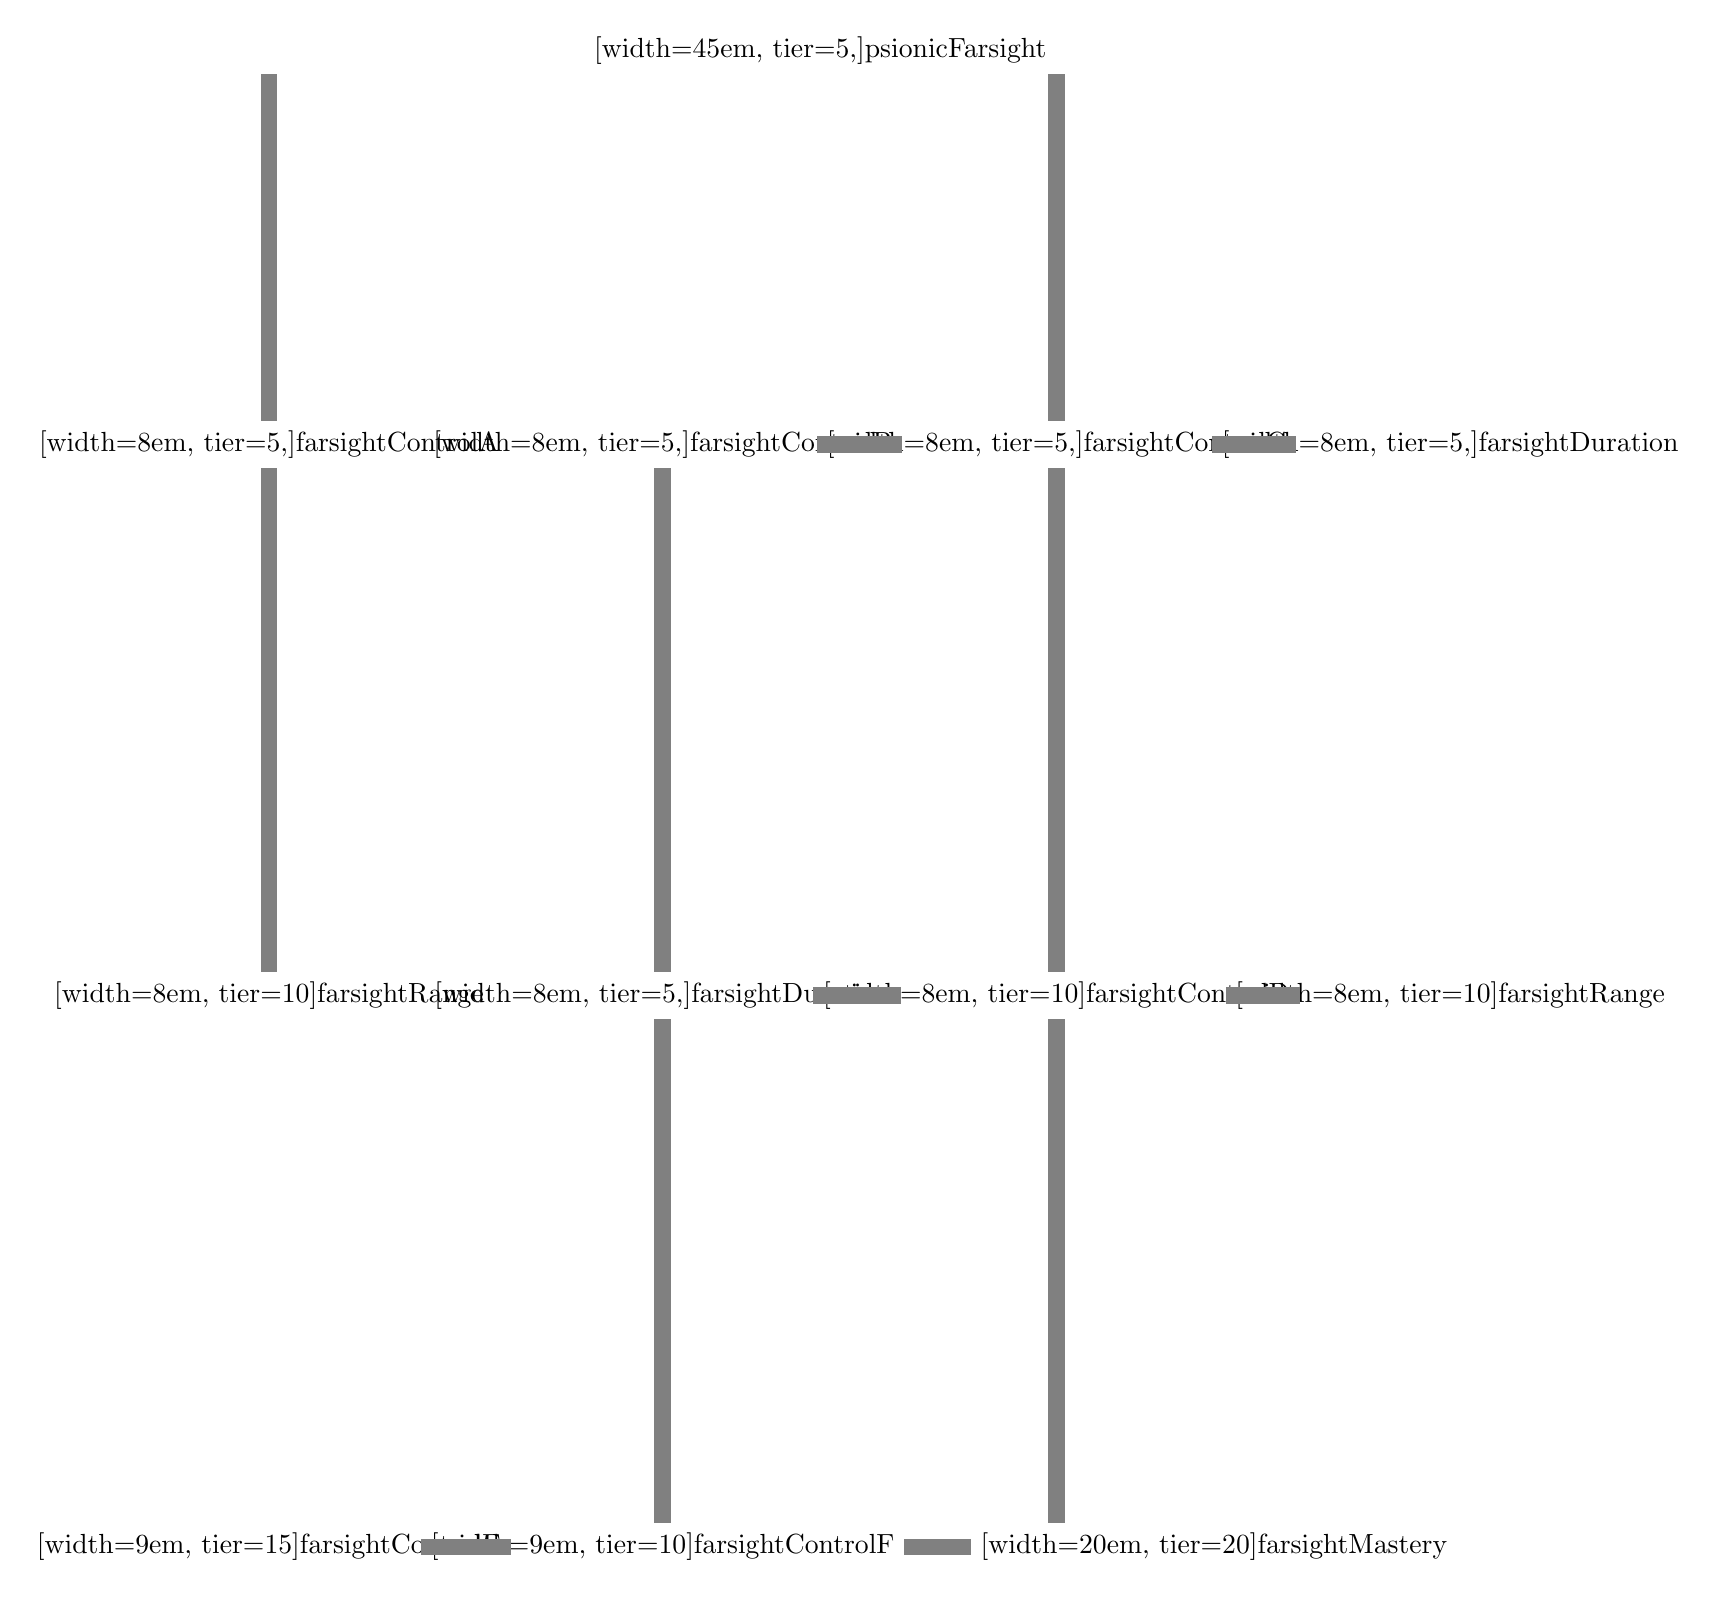
\begin{tikzpicture}
    \draw (-13,   5) node(pr){\TalentBox[width=45em, tier=5,]{psionicFarsight}};
    \draw (-20,   0) node(aa){\TalentBox[width=8em,  tier=5,]{farsightControlA}}
          (-15,   0) node(ab){\TalentBox[width=8em,  tier=5,]{farsightControlB}}
          (-10,   0) node(ac){\TalentBox[width=8em,  tier=5,]{farsightControlC}}
          ( -5,   0) node(ad){\TalentBox[width=8em,  tier=5,]{farsightDuration}}
          (-20,  -7) node(ba){\TalentBox[width=8em,  tier=10]{farsightRange}}
          (-15,  -7) node(bb){\TalentBox[width=8em,  tier=5,]{farsightDuration}}
          (-10,  -7) node(bc){\TalentBox[width=8em,  tier=10]{farsightControlD}}
          ( -5,  -7) node(bd){\TalentBox[width=8em,  tier=10]{farsightRange}}
          (-20, -14) node(ca){\TalentBox[width=9em,  tier=15]{farsightControlE}}
          (-15, -14) node(cb){\TalentBox[width=9em,  tier=10]{farsightControlF}}
          ( -8, -14) node(cd){\TalentBox[width=20em, tier=20]{farsightMastery}}
    ;

    \tikzstyle{bar}=[gray,-,>=stealth, line width=6pt]

    \draw [bar] (aa) -- (aa |- pr.south);
    \draw [bar] (ac) -- (ac |- pr.south);
    \draw [bar] (aa) edge (ba);
    \draw [bar] (ab) edge (bb);
    \draw [bar] (ac) edge (bc);
    \draw [bar] (ab) edge (ac);
    \draw [bar] (ac) edge (ad);
    \draw [bar] (bb) edge (cb);
    \draw [bar] (bc) -- (bc |- cd.north);
    \draw [bar] (bb) edge (bc);
    \draw [bar] (bc) edge (bd);
    \draw [bar] (ca) edge (cb);
    \draw [bar] (cb) edge (cd);
\end{tikzpicture}
